% -----------------------------------------------------------------
% Document class: Article
\documentclass[ a4paper, twoside, 11pt]{article}
\usepackage{../../../macros-general}
\usepackage{../../../macros-article}
% Number of the handout, quiz, exam, etc.
\newcommand{\numero}{03}
\setcounter{numero}{\numero}

% -----------------------------------------------------------------
\begin{document}
\allowdisplaybreaks

\begin{center}
\Large Mec\'anica Vectorial (MECG-1001): Trabajo Aut\'onomo \numero \\[2ex]
\small \textbf{Semestre:} 2017-2018 T\'ermino II \qquad
\textbf{Instructor:} Luis I. Reyes Castro \qquad
\textbf{Paralelo:} 08
\end{center}
\fullskip

% =============================================
\begin{problem}
En el siguiente armaz\'on de cuatro piezas el peso $W = 8$ kN. Determine: 
\begin{itemize}
\item \textbf{[1 Punto]} La fuerza que el eslab\'on $AB$ ejerce sobre la barra $BC$ en $B$. 
\item \textbf{[1 Punto]} La fuerza de compresi\'on o tensi\'on en el pist\'on $DF$. 
\item \textbf{[2 Puntos]} La fuerza que la placa $CDE$ ejerce sobre la barra $BC$ en $C$. 
\item \textbf{[2 Puntos]} La reacci\'on de la placa $CDE$ en $E$. 
\end{itemize}

\begin{figure}[htb]
\centering
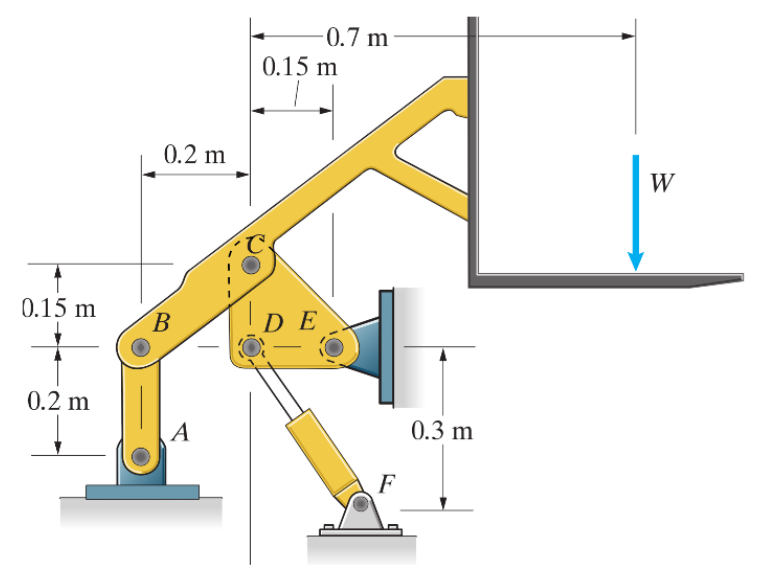
\includegraphics[width=0.56\textwidth]{problema-1.jpg}
\end{figure}

\end{problem}
\fullskip
\fullskip

% =============================================
\begin{problem}
\textbf{[2 Puntos]} En el siguiente cable todos los pesos $W$ son id\'enticos. Determine las distancias verticales $h_2$ y $h_3$. 

\begin{figure}[htb]
\centering
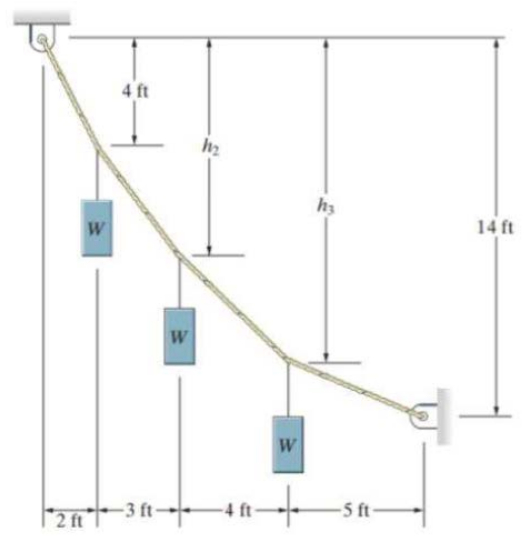
\includegraphics[width=0.5\textwidth]{problema-2.jpg}
\end{figure}

\end{problem}
\fullskip

\end{document}